\documentclass[12pt]{article}
\usepackage{graphicx}
\graphicspath{ {./images/} }
\begin{document}

\section{Week 1 - Linear Regression}
\section{Introduction}
We come across  machine learning all the time 

It's why I don't have to sift through these emails in my inbox

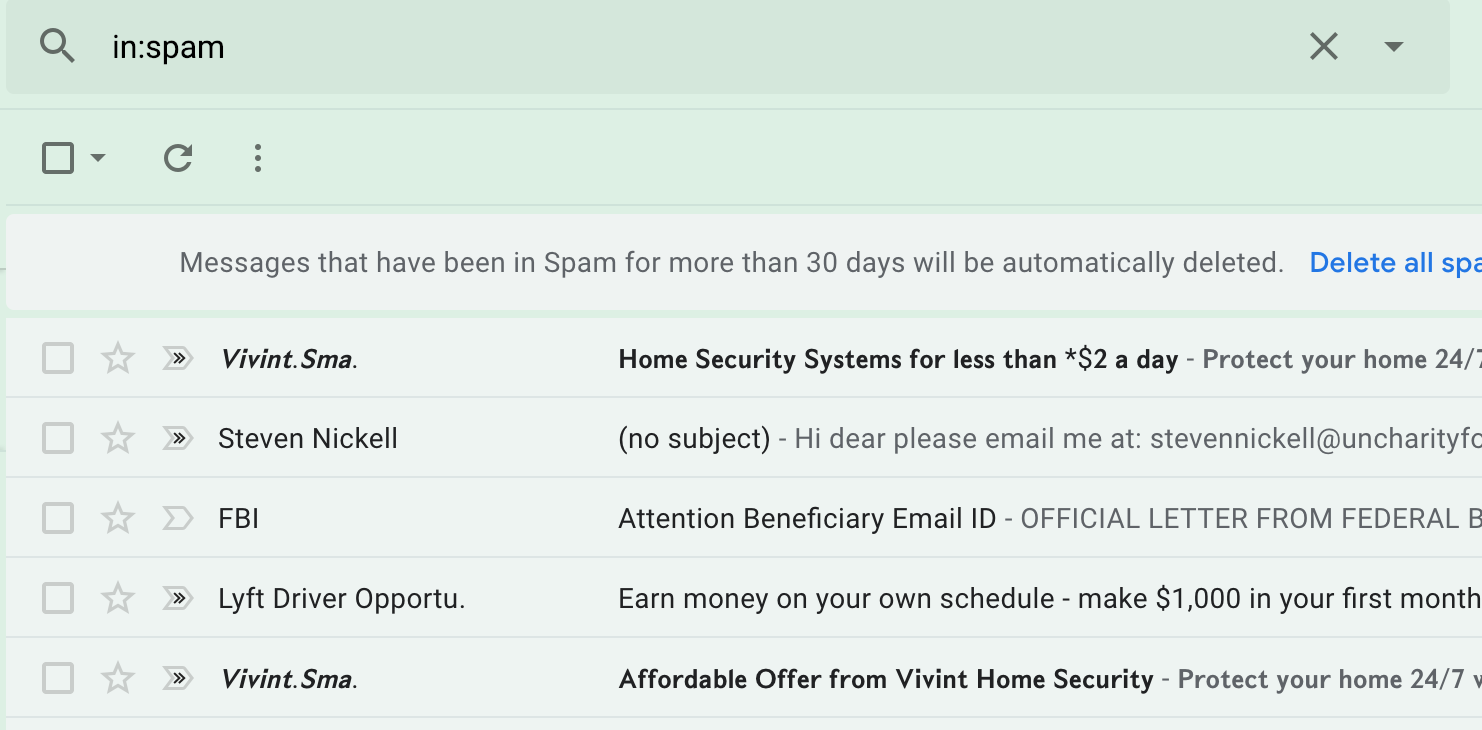
\includegraphics[width=\textwidth]{spam}

It's why I can search my photos, by photos

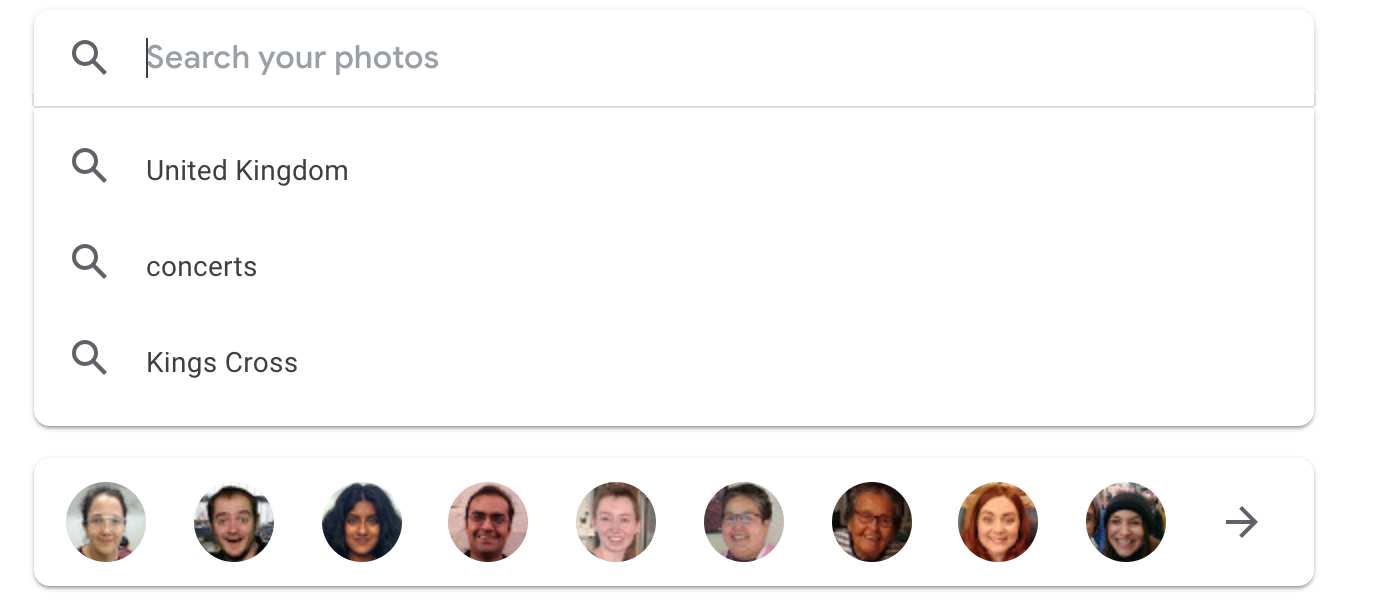
\includegraphics[width=\textwidth]{photo-search}

\subsection{What is Machine Learning?}

According to wikipedia:
Machine learning (ML) is the scientific study of algorithms and statistical models that computer systems use to 
effectively perform a specific task without using explicit instructions, relying on patterns and inference instead.


Machine learning algorithms can learn to do a particular task without being explicitly programmed by building a 
mathematical model based on sample data, known as "training data". Then, that model can be applied to new data 
not previously used to build the model. 

\subsection{What is an algorithm?}

An algorithm is often described as a set of steps to accomplish a particular task. You could describe an algorithm for brushing your teeth, or making a grilled cheese sandwich 

But it's a bit more general than just a set of steps 

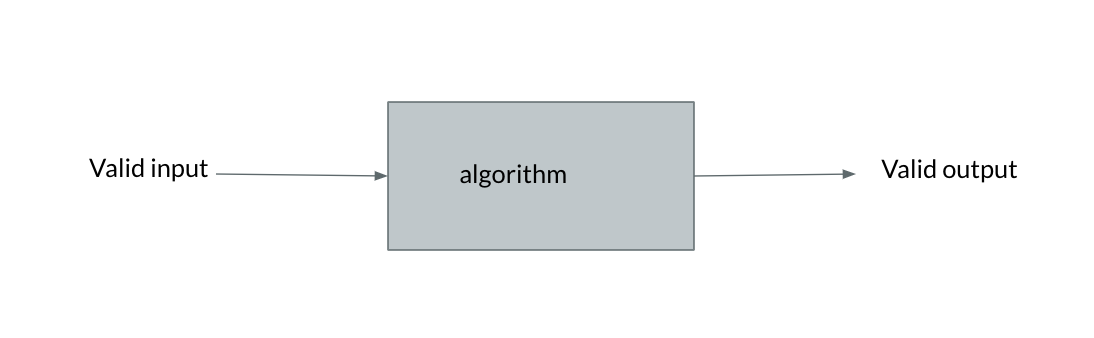
\includegraphics[width={\textwidth}]{algo-abstract}


An algorithm is a way to solve a computational problem, and a computational problem just specifies valid input and desired output. 

For example, for the problem of spam filtering the input would be an email message, and the output would be a 
classification (spam/not spam). The algorithm could be a set of steps. We could compose a series of regular expressions to 
the message that are based on previous messages that we know have turned out to be spam. 

We could also train a model based on a dataset of emails and classifications, to learn patterns of what spam messages 
look like without explicitly writing spam identification rules. Then, we could use the model for new data without a 
classification. That's the approach we're more interested in here, but both approaches are algorithms.

\subsection{What is a machine learning algorithm?}


The ML Coursera course defines a *Well Posed Machine Learning Problem* 

A computer program is said to learn from experience *E* with respect to some task *T* and some performance measure *P* 
if its performance on *T*, as measured by *P* improves with experience *E*

So, we can see that the rule based spam filtering approach wouldn't be a machine learning based approach because having 
more labelled data would not help us to classify spam any more accurately. 

\section{What is a machine learning algorithm?}

Suppose we want to be able to predict someone's weight given their height. 

We start with a data set of height and weight pairs

\end{document}